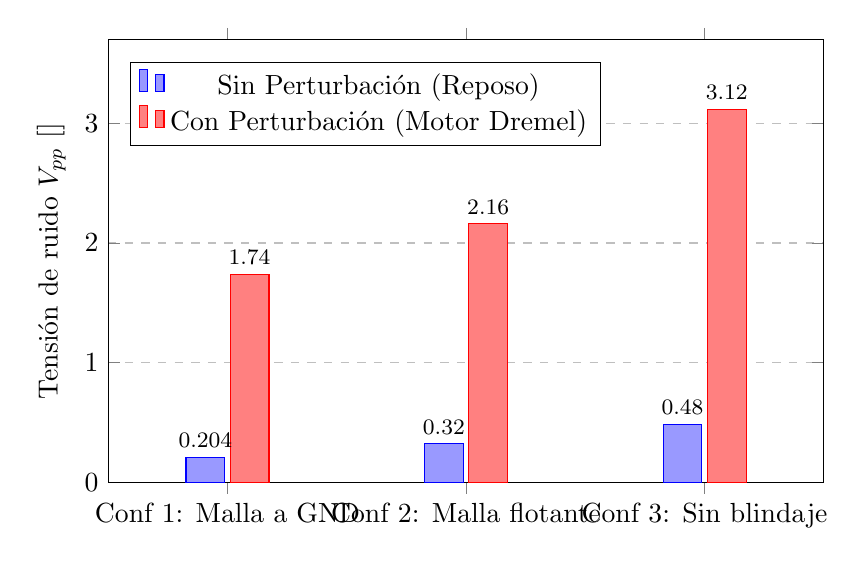
\begin{tikzpicture}
    \begin{axis}[
        ybar,
        bar width=14pt,
        width=0.88\textwidth,
        height=7.2cm,
        ylabel={Tensión de ruido $V_{pp}$ [$\unit{\volt}$]},
        symbolic x coords={Conf 1: Malla a GND, Conf 2: Malla flotante, Conf 3: Sin blindaje},
        xtick=data,
        nodes near coords,
        nodes near coords style={font=\footnotesize, /pgf/number format/fixed, /pgf/number format/precision=3},
        ymin=0,
        ymax=3.7,
        legend style={at={(0.03,0.95)}, anchor=north west},
        ymajorgrids=true,
        grid style=dashed,
        enlarge x limits=0.25
    ]
        \addplot[fill=blue!40, draw=blue] coordinates {
            (Conf 1: Malla a GND, 0.204)
            (Conf 2: Malla flotante, 0.320)
            (Conf 3: Sin blindaje, 0.480)
        };
        \addplot[fill=red!50, draw=red] coordinates {
            (Conf 1: Malla a GND, 1.740)
            (Conf 2: Malla flotante, 2.160)
            (Conf 3: Sin blindaje, 3.120)
        };
        \legend{Sin Perturbación (Reposo), Con Perturbación (Motor Dremel)}
    \end{axis}
\end{tikzpicture}
